\chapter{Background}
\label{background}
\section{Infandango}
Infandango is an automated web-based marking system for student submitted programming exercises. A student can view the list of warm-up, optional and core exercises and choose to submit a file for one of them. This file is then compiled and tested by Jester in a sandbox. Between the web frontend and Jester there is a PostgresSQL database which stores which files have been submitted for which users and how these files performed on the JUnit tests.
\subsection{Current feedback}
The primary source of feedback in Infandango is displayed in Figure \ref{fig:currentfeedback}. Each submissions is marked with a set of JUnit tests and the fraction of these tests which are correct is displayed. This fraction is converted into a percentage and displyed on a green or red background depending on the value. %EPLXAINT HTIS LOL
More general feedback is also available which displays similar information but the results are displayed by week rather than by question. 

\begin{figure}[p]
\centering
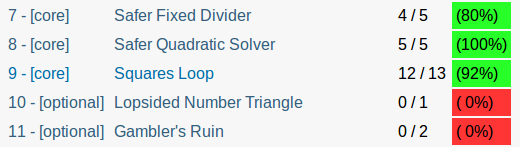
\includegraphics[width=0.8\textwidth]{currentfeedback.png}
\caption{This is a crop of what will be displayed to the user for a given week}
\label{fig:currentfeedback}
\end{figure}

\section{Literature}
Khan Academy\cite{khan_site} is a website which provides users with online education material:
\begin{quote}
Our online materials cover subjects ranging from math and finance to history and art.  With thousands of bite-sized videos, step-by-step problems and instant data\cite{ka_faq}
\end{quote}
A blog post\cite{khan_blog} written by David Hu about Khan Academy demonstrates that different feedback measures can affect user performance significantly. The original Khan Academy system required a user to get 10 consecutive exercises of a certain type correct before they can be deemed proficient\footnote{A proficiency is earned when a user is deemed to be "proficient" at a certain kind of exercise} at that type of exercise. In an attempt to improve this system, a logistic regression model is used to calculate the probability that a user passes the next exercise successfully, with a threshold of 94\% representing the new proficieny level. Over a 6 day period 10\% of users tested the new method. Users of the new system earned 20.8\% more proficiences, attempted 15.7\% more exercises and required 26\% less exercises per proficiency. Hu summarises by saying the boost seems to come from allowing users to move on from exercises which they already proficient at, without requiring them to complete their streak thus wasting time on something they already understand.
